% Chapter 1

\chapter{The basic safety hypervisor} % Main chapter title

\label{Chapter2} % For referencing the chapter elsewhere, use \ref{Chapter1} 

%----------------------------------------------------------------------------------------

% Define some commands to keep the formatting separated from the content 
%\newcommand{\keyword}[1]{\textbf{#1}}
%\newcommand{\tabhead}[1]{\textbf{#1}}
%\newcommand{\code}[1]{\texttt{#1}}
%\newcommand{\file}[1]{\texttt{\bfseries#1}}
%\newcommand{\option}[1]{\texttt{\itshape#1}}

%----------------------------------------------------------------------------------------

% IMPORTANT Add a section about IPC and inter-partition communication
% IMPORTANT Do I talk enough about whether or not developers offer para or full or both?
% IMPORTANT Talk about supported hardware, v7 vs. v8 and breadth of platforms

% IMPORTANT Maybe remove the intro fluff?
Now that the differences between traditional hypervisors and embedded safety hypervisors have been laid out, it is time to take a closer look at the embedded safety hypervisor.
For this purpose, a "basic safety hypervisor" will be proposed that embodies the typical characteristics of a microkernel-based safety hypervisor. Where there is no discernible consensus, differences will be highlighted. Both the typical hypervisor architecture and its simplified functionality will be examined.
The information in this chapter has been collected by analyzing the manuals of open-source safety hypervisors and industry white papers \cite{okl4manual} \cite{xtratum3} \cite{sel4faq} \cite{pikeosscheduling} \cite{masmano2009xtratum}. 

\section{Architecture}
Since most safety hypervisors are microkernel-based, the architecture for the basic safety hypervisor is also a more in-depth look at microkernel architecture. However, there are differences and additions to the microkernel core that will be explored as well.   

The guiding principle of microkernel design, minimality, has already been introduced in section \ref{microkernel}. However, while the academic microkernel representations try to achieve \keyword{absolute minimality}, most real safety hypervisor implementations forego this to add useful features to the kernel. The small trusted code base is still an integral part of safety hypervisors, but with some minor trade-offs. 

% SOURCE Do I need a source for this?
Perhaps, the most significant trade-off is the inclusion of the virtual machine monitor code in the kernel itself. Some hypervisors also relegate this virtual machine control to user-space, but it is more typical to see it inside of the microkernel. In reality, the virtualization aspect of the hypervisor is almost always a critical component, and it, therefore, makes sense to include it in the kernel verification efforts. 

\subsection{Capability-based access control} \label{sec:capability-based_ac}
% TODO Explain concept of least privilege
Capabilities are unforgeable tokens that grant access rights to an object. They contain the identification of the object and associated rights, for example, read and write.
They can be given to other processes which in turn grants them access according to the capability \cite{levy1984capability}. A capability could be for a specific memory region, a communication endpoint or to a hypervisor \acrshort{api} call.

The capabilities a process has, are maintained in a part of memory that it can not write, to stop the process from attempting to forge capabilities. It is however still up to the process to use the appropriate capability for access to reduce kernel involvement. In practice, this means that the process will request access by pointing to his corresponding capability in kernel memory. The kernel then checks the capability, and if it does indeed grant access to the requested rights, the kernel approves the request. If it was not the responsibility of the user process to know the right capability, the kernel would have to be extended with code that looks up the capabilities of a process. But this would violate the microkernel's principle of minimality.

Capability-based access control has dominated in microkernels because of its flexibility and because it does not require extensive kernel involvement. Since the typical safety hypervisor is an extension of a microkernel, this mechanism has propagated to them as well and is typically seen in extensive configuration files.

\subsection{Scheduling} \label{hv-scheduling}
All hypervisors implement some form of hierarchical scheduling, where a container task is scheduled that then schedules its children according to a global scheduling algorithm. This is most evident with virtualized operating systems. The hypervisor schedules the virtualized operating system according to the system configuration but how the \acrshort{os} in turn schedules its processes is up to the \acrshort{os}. Hierarchical scheduling can have the benefit of reducing scheduling slack in mixed criticality systems \cite{mollison2010mixed}. 

When it comes to how the container tasks are scheduled there is no single solution that is effective for every scenario. Consequently, the basic safety hypervisor offers different configurable scheduling behaviors. The two most common scheduling algorithms are preemptive priority-based scheduling and time-sliced round-robin scheduling. Regardless of which algorithm is used, it needs to be deterministic to enable \acrlong{wcet} analysis. Without deterministic scheduling and \acrshort{wcet} analysis temporal separation cannot be guaranteed, and the system is unable to satisfy real-time requirements verifiably.

\paragraph{Preemptive priority based scheduling}
% FIGURE This might need one
In preemptive priority-based scheduling, each process has a priority and processes that are ready to be scheduled are scheduled based on their priority.
The preemptive in the name means that, if a process with a higher priority than the currently running process becomes ready to be executed, the currently running process gets interrupted. This ensures that the most critical task always gets the time it needs. If there are multiple processes with the same priority, the first to arrive gets scheduled first.

\paragraph{Time-sliced round-robin scheduling}
In time-sliced round-robin scheduling each process gets a dedicated time slice called a quantum. Figure \ref{fig:round_robin_example}  shows an example with three processes and their associated scheduling windows. If the end of the quantum is reached before the process is done, it gets interrupted and the next process is scheduled.
\begin{figure}[ht!]
\centering
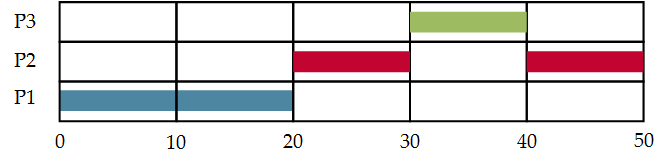
\includegraphics[scale=0.75]{Figures/round_robin_example.png}
\decoRule
\caption{An example for round robin scheduling}
\label{fig:round_robin_example}
\end{figure}

However, these were just the two most prevalent examples, and in fact, most hypervisors even allow the implementation of custom scheduling algorithms, if the provided ones are not sufficient.

Another feature of the basic safety hypervisor is the possibility of multiple scheduling plans. A hypervisor partition with the correct capabilities is allowed to switch the scheduling behavior to one of the plans that were provided at configuration time. For example, if there is an unexpected error, the monitoring partition can put the device into a maintenance mode, where only the most critical and recovery processes are scheduled. Another use for this feature is during the boot process where some partitions might need to run uninterrupted for a longer time.

\subsubsection{Multicore support}
Multicore has been much sought after feature in safety-critical device development. However, traditional processors are difficult to use in safety-critical devices. 
One big problem is presented by the shared cache between cores.

Imagine a system with two partitions, one safety-critical one non-critical, that runs on a two-core \acrshort{cpu} with a shared cache between the two cores. During its allocated time, the safety-critical partition may fill up the cache with relevant values. Once the non-safety-critical software runs, it can evict all of the cache values by populating it with its own values. The resulting cache misses can lead to substantial and potentially unpredictable interference across domains \cite{biondi2018challenges}.

In the best case, this scenario just leads to an excessively pessimistic \acrfull{wcet} analysis. To compensate this, the safety-critical partition would get a lot more allocated time than it needed, leading to a worse average case performance. However, there are efforts to solve this issue reliably. One approach is to adjust the hypervisor to ensure safe cache usage \cite{modica2018supporting}. Another approach is focused on changing processor design to prevent unsafe, non-deterministic cache management in the first place \cite{el2013across}.

Figure \ref{fig:multicore} shows how multicore support is realized in the hypervisor. Each physical core can be assigned to one or more virtual cores, but each virtual core can only be assigned to one physical core. Scheduling plans are then defined for each physical core. To the partitions, the virtual cores appear just like normal cores. This approach ensures temporal determinism.

Currently, handling the cache safely is left to the partitions in most hypervisors. This typically results in the cache being flushed at the beginning of execution or disabled entirely. Naturally, this is inefficient, but safety is more important than performance in most cases.

\begin{figure}[hb!]
\centering
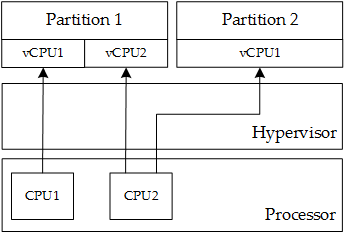
\includegraphics[scale=1]{Figures/multicore.png}
\decoRule
\caption{Multicore assignment example}
\label{fig:multicore}
\end{figure}

\subsection{Available guest environments}
\subsubsection{\acrshort{rtos}}
Any safety hypervisor can host a \acrlong{rtos} as a guest environment, as it is one of the core objectives to separate real-time, safety-critical domains from the less critical domains. However, as explained in section \ref{hw-virt} (Hardware virtualization) the full virtualization of operating systems is not always available or feasible, and in fact, many hypervisors do not currently offer full virtualization. That leaves paravirtualization as the only option, but paravirtualization requires the modification of the operating system in question. To reduce the barrier of entry the developer of the basic safety hypervisor typically also offers an already paravirtualized \acrshort{rtos} that can be deployed on the hypervisor. 

However, this significantly reduces the possible \acrshort{rtos} options the safety-critical device manufacturer can choose for his application. Since most real-time operating systems are closed source, they cannot be modified to work on the hypervisor. This makes the \acrshort{rtos} provided by the hypervisor developer the potentially only viable option and therefore increases the dependence on the developer. What the potential consequences of this are, needs to be evaluated based on the context of the situation but it is an important aspect to keep in mind.

\subsubsection{Linux}
An already paravirtualized version of Linux is another standard guest environment. Since Linux is open-source the pressure of paravirtualization is not an immediate issue. Furthermore, there is less of a difference between versions of Linux than between real-time operating systems by different vendors. It is therefore unlikely that the safety-critical device manufacturer is even interested in using another version than the one provided.

\subsubsection{Native C runtime environment}
For a partition completing a very simple task, running a full-blown operating system is a waste of resources. For that reason, the basic safety hypervisor includes a guest environment that is nothing more than a native C application with access to the hypervisor \acrshort{api}. The safety-critical device manufacturer can provide one or multiple C files that then get compiled into a hypervisor process. This process is then scheduled like any of the other partitions.

A possible application of this is a shared device driver. The driver can be implemented in the native C environment and communicate with the other partitions over the hypervisors \acrshort{ipc} mechanism. A more detailed explanation of this scenario will be given in a future section.

%----------------------------------------------------------------------------------------

\section{Functionality}
This section will explore what functionality the safety hypervisor can offer and what the basics of their implementation are.
\subsection{Hardware access}
Ultimately, the hypervisor partitions need to be able to interact with the hardware in some form. Access to the partition's assigned physical memory regions is established by the \acrshort{mmu} in the form of virtual memory.
To communicate with its assigned peripherals, the partition needs access to the peripheral device registers, and it needs to be notified when the peripheral triggers an interrupt. How the hypervisor deals with the special case of \acrfull{dma} will also be explained.

\paragraph{Device register access}
% TODO Is this true?
In Intel \acrshort{cpu}s device registers are often accessed via \acrshort{io} ports. For simplicity's sake only the model typical for many other processors, memory mapped \acrshort{io}, is examined. With memory mapped \acrshort{io} the peripheral device registers get mapped into the physical address space. That means a process that can read this memory location is reading the contents of the device register. Similarly, a process that writes to this memory location is modifying the device register that is mapped to it. Consequently, to give a partition the ability to interact with the registers of a peripheral device the hypervisor simply needs to give access to the corresponding memory regions. This can be configured through the \acrshort{mmu} as explained previously.

\paragraph{Interrupts}
Interrupts are the asynchronous way for peripheral devices to communicate with the \acrshort{cpu}. Every peripheral has an associated interrupt line to the interrupt controller. Once the peripheral wants to signal the \acrshort{cpu} it wants to communicate, it activates its interrupt line. Then the interrupt controller buffers this interrupt request and forwards it to the \acrshort{cpu} which interrupts its current execution to handle the interrupt. Then the \acrshort{cpu} can notify the kernel via the interrupt handler code that is assigned to the number of the interrupt line that was just activated. The interrupt handler is responsible for retrieving the data from the device registers and preparing the peripheral for the next communication.

In a fully virtualized guest, the hypervisor can utilize the hardware virtualization extensions to trap an interrupt request and send a virtual interrupt to the partition. Another option that also works without the virtualization extensions is interrupt pass-through. In the pass-through scenario, the hypervisor simply routes the interrupt to the interrupt handler in the partition and the partition has to take care of everything else.

% TODO Is this true?
In any case, the partitions cannot be allowed to gain unmitigated access to the interrupt controller. The hypervisor makes sure that only the interrupts assigned to the partition during configuration are routed to that partition. Furthermore, it prevents the partitions from disabling the interrupts they do not have permission for. Without these restrictions, partitions could breach the separation the hypervisor sets out to achieve.

\paragraph{\acrshort{dma}}
% TODO Include a source for IOMMU
A special case of peripheral to process communication is that of \acrfull{dma}. \acrshort{dma} means that a peripheral device independently accesses the system memory without \acrshort{cpu} involvement. This can be drastically faster and relieves the load on the \acrshort{cpu} but poses a special problem for safety-critical devices. Because the hypervisor cannot know \acrshort{dma} activity, a misbehaving or hijacked peripheral device can write to potentially arbitrary memory locations. The only way to relieve this is with the help of an \acrfull{iommu}. A hardware component that, like an \acrshort{mmu}, can restrict the memory regions a peripheral can access via \acrshort{dma}.
If this is not present, \acrshort{dma} should likely be disabled.

\subsubsection{Shared hardware access}
If the hardware virtualization extensions are present in the \acrshort{cpu}, the hypervisor can arbitrate access to most devices by presenting virtual devices to the partitions.
However, an interrupt line can only be directly assigned to one partition, so if the direct assignment of the hardware is necessary, shared access needs to be realized differently. 

\begin{figure}[hbt!]
\centering
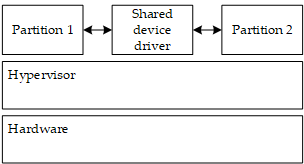
\includegraphics[scale=0.8]{Figures/shared_driver.png}
\decoRule
\caption{High level view of an \acrshort{io} server partition}
\label{fig:shared_driver}
\end{figure}
Figure \ref{fig:shared_driver} depicts how this is typically done. The peripheral in question gets assigned to a hypervisor partition that acts as an \acrshort{io} server for the other partitions. Any partition that wants to use this peripheral can communicate with the \acrshort{io} server partition over the hypervisor \acrshort{ipc} mechanism, which is represented here by the arrows between partitions. How access is granted and arbitrated between partitions is up to the implementer. It is important to note that these kinds of drivers do not typically come with the hypervisor and it is up to the device manufacturer to implement them.

\subsection{Inter-partition communication}
There are two ways for two partitions to communicate: message passing and shared memory.

\subsubsection{Shared memory}
\begin{figure}[hbt!]
\centering
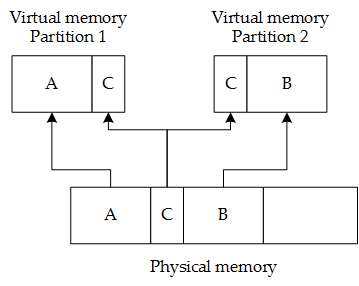
\includegraphics[scale=0.8]{Figures/shared_memory.png}
\decoRule
\caption{Shared memory between two partitions}
\label{fig:shared_memory}
\end{figure}
If two partitions are configured to share memory, the hypervisor simply maps the same region of physical memory into the virtual address space of both partitions. Figure \ref{fig:shared_memory} shows that partition 1 and 2 both get access to the physical memory region C. In this example there is still some unmapped physical memory after memory region B. 

It is up to the partitions to know how the data in the shared region needs to be interpreted and to synchronize access on the region. The hypervisor does not control access can therefore not guarantee that none of the partitions corrupts the memory. Consequently, this way of communication provides a lot of flexibility at the cost of safety.
One way to get around the concurrency issues is to make memory access in this region read-only for one of the partitions.

\subsubsection{Message passing}
Message passing is the safe way for two partitions to communicate that relies on the hypervisor's \acrshort{ipc} mechanism. A communication channel is a unidirectional path between one source and one or more destinations. The partitions can access a channel through ports, of which there are two types. Queuing ports maintain a \acrshort{fifo} queue of messages that can be read by the receiving partitions sequentially. In a sampling port, there is only ever one message that either gets overwritten by a new message or invalidated by the partition reading the message. To make the polling of the ports unnecessary, the hypervisor triggers a specific interrupt in the receiving partitions when a new message is available.

Figure \ref{fig:message_ports} shows an example of communication between three partitions. 
Messages sent by partition 1 arrive at the ports in partition 2 and 3 individually. That means messages are maintained on a port by port basis and a partition cannot stop another partition from receiving the message by consuming it. The hypervisor also ensures that messages either arrive completely or not at all, where "not at all" would trigger an error. All message data is copied by the hypervisor, and there is no direct memory access to the original message. Therefore, partition 1 can't change the message after it has been sent to the other partitions. These assurances can only be made by the hypervisor because it has full control over the communication, unlike the shared memory communication.

All communication ports and channels need to be defined at configuration time. Once the system is compiled and running no ports or channels can be created that weren't already in the hypervisor configuration. This allows safety-critical device manufacturer to reason about the dependence between partitions.
\begin{figure}[hb!]
\centering
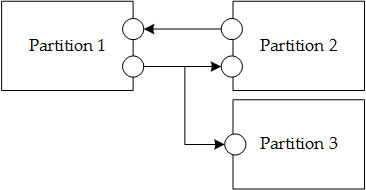
\includegraphics[scale=0.8]{Figures/message_ports.png}
\decoRule
\caption{Message ports between three partitions}
\label{fig:message_ports}
\end{figure}


\subsection{Health monitoring}

\begin{figure}[hb!]
\centering
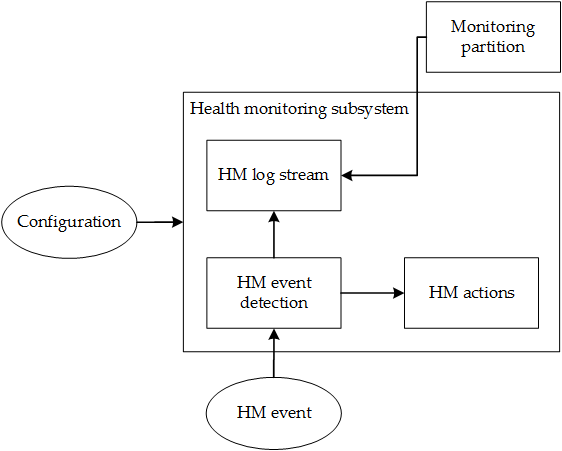
\includegraphics[scale=0.75]{Figures/health_monitoring.png}
\decoRule
\caption{High-level view of the health monitoring subsystem}
\label{fig:health_monitoring}
\end{figure}
% TODO Example?
Apart from virtualization, health monitoring is likely the most interesting hypervisor feature for safety-critical device manufacturers. Health monitoring is a subsystem of the hypervisor that monitors and reacts to abnormal system behavior. This is possible due to the hypervisor's complete view of the system.

% TODO Are these examples clear?
There are three types of events the health monitoring system can recognize: First, are events that are triggered by abnormal hardware behavior. Some examples of this are division by zero and attempted access to a protected memory region. The hypervisor gets notified of abnormal hardware behavior by processor exceptions.

The second type of event is triggered by the code running in a partition. These are typically caused by failed assertions. 

The final event type is triggered by the hypervisor itself. This is typically a response to a violation of the hypervisor configuration. For example, a partition that tries to create an \acrshort{ipc} port that has not been defined in the configuration or a partition that attempts to use a hypercall it does not have permissions for.

Figure \ref{fig:health_monitoring} depicts a high-level view of the health monitoring subsystem. This figure is a modified version of the health monitoring image in \cite{xtratum3}. Health monitoring is split into three parts: event detection, automated actions, and the health monitoring log stream. The behavior of the entire subsystem is dictated by the hypervisor configuration.
After an event has occurred, it gets recognized by the event detection component. Then, depending on the hypervisor configuration, an automatic action may get triggered. Possible actions are:
\begin{enumerate}
    \item Ignore the event.
    \item Shut down the offending partition.
    \item Reset the offending partition.
    \item Shut down the entire system.
    \item Reset the entire system.
    \item Forward the event to the offending partition as a virtual interrupt.
\end{enumerate}

If the event is configured to create a log entry it then gets written to the health monitoring log stream. The entry contains information about the offending partition and relevant information about the event itself. In figure \ref{fig:health_monitoring} there is a hypervisor partition, called "monitoring partition" that has access to the log stream. If the predefined actions are not capable of resolving the issue, this monitoring partition can take further actions. Whatever this partition does with the information is up to the device manufacturer, but an example would be to put the device into a maintenance mode, where only the most critical partitions are scheduled. 

\subsection{Timers}
To aid the partition with time management, the hypervisor offers two clocks. One is the elapsed microseconds since the last device reset and the other is the partition execution clock for every partition. The partition execution time is maintained on a per-partition basis and only advances when the respective partition is being executed.

Partitions can request the current time and also arm a timer for each clock. Once this timer elapses the partition receives a virtual interrupt by the hypervisor. 
\subsection{Partition privileges}
Capabilities have already been introduced in section \ref{sec:capability-based_ac} to show how privileges are assigned to partitions. But only some basic examples of what privileges there are have been given. 

At the most, basic level partitions can be split into two categories: system partitions and normal partitions \cite{xtratum3}. Normal partitions have access to all their resources like interrupt lines, memory regions and message ports. They are also allowed to use hypercalls that can not disrupt the system at large, like accessing timers or retrieving the current system status.

System partitions have access to all their assigned resources, and on top of that, they can call hypercalls that can impact the entire system. They can change scheduling plans, access the health monitoring log and even start and stop other partitions. Naturally, system partitions need to be trusted by the safety-critical device manufacturer because they have the capabilities to stop the system from functioning correctly.

Most hypervisors offer more granular distinction than normal partitions and system partitions, where individual hypercalls can be enabled or disabled for specific partitions.
\subsection{Static configuration}
Throughout this chapter, the role of the hypervisor configuration has already been highlighted. In this section, it will be summarized which aspects of the system can be controlled with the hypervisor configuration and what core principles it is based on. The configuration file is typically in the form of an \acrshort{xml} document that acts as input for the creation of the final hypervisor executable image.

The configuration file can be used to define the following aspects of the system:
\begin{itemize}
    \item Partitions and their associated binaries.
    \item Hardware resource access of partitions.
    \item Scheduling behavior.
    \item Partition rights.
    \item Inter-partition communication paths.
    \item Health monitoring.
\end{itemize}

Any configuration of the hypervisor and its subsystems are static and explicit. Static means everything has to be defined before the binary has been compiled and deployed. A communication path that can not be found in the configuration file can also not be created at runtime. Explicit configuration refers to the default level of privilege of the partitions. A system designer needs to explicitly define every permission of each partition in the configuration file. This avoids unintended access to potentially disruptive functionality. Exempt from this explicit access are some functions that are entirely unable to disrupt other partitions, like accessing the current hardware time.

\subsection{Separation}
% IMPORTANT What about the other requirements of a sep-arch?!
The concepts of separation have been introduced in section \ref{separation-arch}. In this chapter, there have also already been mentions to the hypervisor assurance in regards to certain subsystems. For example, the assurance that messages are copied to all destination ports correctly or an appropriate error is triggered. They have already been part of the hypervisors separation assurances. Now it is time to take a more specific look at how the hypervisor satisfies the most crucial requirements of a separation architecture. 

\subsubsection{Temporal separation}
How the hypervisor may schedule its partitions has already been explained in section \ref{hv-scheduling}. The most important property of a hypervisor scheduling algorithm that emerged from that was its determinism. If the algorithm is deterministic, the device manufacturer can carry out a \acrshort{wcet} analysis, which allows him to reason about the device's temporal separation. The results of the \acrshort{wcet} analysis should show that even in the absolute worst case, the critical partitions still get the time they need to fulfill safety-critical functions. In all highly critical devices with real-time requirements, this is a necessary step to achieve regulatory compliance.

% TODO Does the interrupt system get disabled during IRQ or not?
Because the hypervisor has full control over the system, it can stop or start processes at will. Through this, the hypervisor can make sure the schedule is kept, and no process oversteps its temporal boundaries.
Additionally, the hypervisor prevents partitions from disabling interrupts they do not have permissions for. This makes sure all partitions always get timely interrupts which is an important aspect of temporal separation. 
\subsubsection{Spatial separation}
Spatial separation is mostly concerned with preventing illegitimate access to memory. Because a hypervisor can only be deployed on a system with \acrshort{mmu} achieving this is fairly simple. The hypervisor configuration details all memory assignments to the partitions and the hypervisor configures the \acrshort{mmu} to only grant access to those assigned regions. 

Another important shared resource is kernel memory. Any objects that shouldn't be accessed directly by a partition are kept in kernel memory. A partition that continuously provokes the hypervisor to create objects in kernel memory could stop all other partitions from using certain hypervisor functionality. To prevent this, the basic safety hypervisor implements a per partition kernel memory quota. Once this quota is depleted, the hypervisor will no longer create kernel objects for this partition.

\acrshort{dma} poses a severe threat to temporal separation and should only be enabled if the device contains an \acrshort{iommu} to regulate and control direct memory access.

%----------------------------------------------------------------------------------------
\section{Initial considerations}
% TODO Rename this section
Although the considerations for choosing a hypervisor implementation will be outlined later in the thesis, i.e., in section \ref{how-to-decide}, some crucial factors need to be elaborated here to avoid confusion.
\subsection{First- or third-party hypervisor}
A manufacturer has the option to either license a third-party hypervisor or develop his own solution. The development costs of a third-party hypervisor are effectively shared with many parties over the course of many projects, whereas the development costs of a first-party hypervisor are typically only shared throughout many projects in a single company. However, developing one's own hypervisor provides the maximum amount of control over functionality and development cycle.

Additionally, it means that the best possible subject matter experts on the hypervisor are always available to the manufacturer. However, here also lies another big problem: Developing a custom hypervisor not only requires the initial development costs but also the costs of hiring or developing the talent required. A third-party already has these capacities and can therefore also typically go beyond the absolute necessity regarding functionality.

Ultimately, the more prudent approach is probably licensing a third-party hypervisor, but in some cases, it may be beneficial to have full control over the environment. 

\subsection{Security}
Security will not be a consideration in this thesis, only a word of warning will be issued. It may seem logical to assume that a hypervisor can provide security as well as safety and while it may not initially be a bad idea to have separation between security-critical and non-security-critical software it is not that simple. A hypervisor offers a much greater attack incentive, as a compromisation of the platform could be used to attack a lot of different devices. It is also questionable whether or not the goals of security and safety align. A manufacturer does not want to modify a certified device or at least do it in bulk to minimize the cost of recertification. Building a secure device on the other hand often requires frequent updates to fix newly found attack vectors. So the security of any given hypervisor implementation should not be taken for granted and analyzed with scrutiny.
%----------------------------------------------------------------------------------------

\section{Limitations}
Before getting into the full-fledged analysis, it is best to expose some limitations of the current safety hypervisor landscape. 
\subsection{Current hardware restrictions}
Hypervisors are overall still limited to the more powerful \keyword{application processors} and have not penetrated the \keyword{microcontroller} market. Using a hypervisor is also not possible if a specialized processor, like a \acrfull{dsp}, will be the only processor in the system. Although, this restriction may be lifted in the future.  There are several reasons for the hypervisor's hardware restrictions. 

% PHRASING 
First of all, microcontrollers typically have no \acrshort{mmu} only an \acrshort{mpu} or no memory protection at all. Hypervisors need at least some hardware memory protection, as the corresponding software isolation is far too slow. \acrshort{mpu}s have a limited number of partitions they can isolate and therefore impose uncomfortable restrictions on hypervisor developers and users.

Second, the hardware virtualization extensions are not yet available on microcontrollers, and even though the typical safety hypervisor prefers paravirtualized guests, virtualization extensions are still beneficial for preventing the guest from doing things it is not supposed to. ARM, for example, offers a trap mechanism that allows the hypervisor to disable certain instructions and special registers for the guest \cite{ARM.v8.2018}. 

And finally, a hypervisor is fundamentally about isolating software components from each other. It is more likely that this is necessary on a stronger processor and not on a microcontroller.

However, with all of these restrictions laid out, there are developments that aim to make hypervisors viable on microcontrollers. Read more about this in section \ref{tech-progress}.




%----------------------------------------------------------------------------------------

